% Nyolcadik, kilencedik és tizedik előadás

\chapter{Buszrendszer}

A buszrendszer egységek közötti kommunikációra szolgál (pl. CPU-MEM-perifériák), a kommunikáció infrastrukturális része.
Egy történeti fejlődés eredménye, az adatkommunikációs megoldások közül ez bizonyult a legjobbnak.
Az első szabványos buszrendszert az IBM hozta létre 1981-ben.
Fontos, hogy ez egy nyílt szabvány volt, minden mai buszrendszernek ez az alapja, tehát minden buszrendszer lényege, hogy szabadon használható, nyílt architektúrára épül.
A szabványok definiálják a vezetékköteget és a csatlakozók kiosztását, a szabványok függetlenek a processzor belső architektúrájától, tehát platformfüggetlen megoldást jelentenek.

\section{Jellemzői}
\begin{itemize}
    \item az eszközök kizárólag ezen keresztül kommunikálnak
    \item egy buszrendszerre általában egyszerre több egység kapcsolódik \textrightarrow meg kell oldani az adatátvitelben részt vevő eszközök kijelölését, meg kell határozni az átvitel irányát és meg kell oldani az összehangolást és szinkronizálást.
    \item a felsorolt problémák megoldására a legfontosabb a szabványosítás - szabványos jelhasználat, vezetékkiosztás
    \item fontos tulajdonsága a sebesség, hogy az adatkommunikáció ne jelentsen szűk keresztmetszetet
    \item a buszrendszer transzparens - a rendszer kezeli, a felhasználó számára nem látható
\end{itemize}

\section{Csoportosítása}
\begin{itemize}
    \item átvitel iránya szerint
    \item átvitt tartalom szerint
    \item átvitel jellege szerint
    \item összekapcsolt területek alapján
    \item átvitel módja szerint
\end{itemize}

\subsection{Átvitel módja szerint}
\begin{itemize}
    \item soros
    \item párhuzamos
\end{itemize}

\subsection{Átvitel iránya szerint}
\begin{itemize}
    \item szimplex (csak egy irányba mehet az adat, pl. címbusz)
    \item félduplex (egyszerre csak egy irányban közlekedik az adat)
    \item duplex (egyszerre két irányba mehet az adat, pl. adatbuszok)
\end{itemize}

\subsection{Átvitel jellege szerint}
\begin{itemize}
    \item dedikált - minden mindennel össze van kötve pl. Intel QuickPath Interconnect
    \item shared (osztott)
\end{itemize}
A megosztott busz egyszerűbb felépítésű, olcsóbb és skálázhatóbb (nem kell mindent mindennel összekötni), de buszvezérlő utasításokra van szükség az ütközések elkerülésére.
Ehhez buszvezérlő vonalakra van szükség.
Hátránya az osztott buszoknak, hogy viszonylag lassúak, bonyolult a vezérlésük és meghibásodás esetén több eszköz kieshet.

\subsection{Átvitt tartalom szerint}
\begin{itemize}
    \item adatbusz
    \item címbusz
    \item vezérlőbusz
\end{itemize}

\subsection{Összakapcsolt területek szerint}
Összekapcsolt területek szerint megkülönböztetünk rendszerbuszt és bővítő (periféria) buszt.
\begin{figure}[H]
    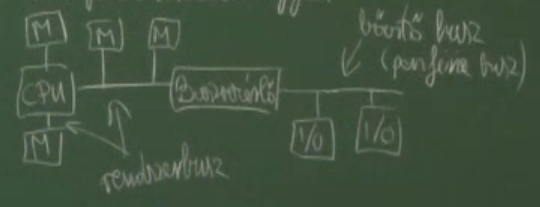
\includegraphics[width=0.8\textwidth]{busz}
    \centering
    \caption{Rendszerbuszok és bővítő buszok}
    \label{fig:busz}
\end{figure}
Bővítő busz pl. a SATA és az USB.

\section{Címbusz}
Ezen a vezetékkötegen áramlik az eszközök címzésére szolgáló adat.

\section{Adatbusz}
A fejlődése során a sávszélességet folyamatosan növelték: 8,16,32,64 bit.
Fokozatos bővítéssel fejlesztettek.

\subsection{Buszvezérlő}
A mai rendszerekben az adatbusz vezetéke közös lehet a címbusszal, időbeli multiplexeléssel.
Ehhez szükség van egy buszvezérlőre és egy vezérlővonalra.
A vezérlőjelek mutatják meg, hogy éppen adat, vagy cím közlekedik a buszon.
A vezérlőjeleket csoportosíthatjuk:
\begin{itemize}
    \item adatátvitelt vezérlő jelek
    \item megszakítást vezérlő jelek
    \item buszvezérlő jelek
    \item egyéb vezérlő jelek
\end{itemize}

\subsubsection{Adatátvitelt vezérlő jelek}
\begin{itemize}
    \item M/IO jelek: megmutatják, hogy memória, vagy IO cím található a buszon
    \item R/W (read/write) jelek: megadja az adatáramlás irányát a CPU felől nézve
    \item WD/B (word/byte): megadja az adat méretét
    \item D/S (data strobe) jel: az adat felhelyezését jelzi a memória számára
    \item A/S (address strobe) jel: a cím buszra helyezését jelzi az eszköz számára
    \item ready jel: az átvitel befejezését vagy a busz rendelkezésre állását jelzi
\end{itemize}

\subsubsection{Megszakítást vezérlő jelek}
\begin{itemize}
    \item megszakítást kérő jelek
    \item megszakítást visszaigazoló jelek
\end{itemize}

\subsubsection{Buszvezérlő jelek}
\begin{itemize}
    \item busz foglalással kapcsolatos jelek
    \item visszaigazolás
\end{itemize}

\subsubsection{Egyéb vezérlő jelek}
\begin{itemize}
    \item reset
    \item CLK
\end{itemize}

\section{Soros és párhuzamos buszok}
Kezdetben soros buszokat alkalmaztak, később párhuzamosak terjedtek el.
A soros busz előnye, hogy kevesebb vezeték szükséges, a párhuzamosoknál viszont hatékonyabb az adatátvitel (egyszerre általában nem 1 bitet kell átvinni, párhuzamos busszal lehetséges több bit átvitele egyidőben).

\section{A PCI szabvány}
A PCI ma a legfejlettebb párhuzamos busz.
Legnagyobb előnye, hogy a PCI buszra csatlakoztatott perifériákat a CPU úgy látja, mintha a saját címterében lenne, azaz mintha azok közvetlenül a rendszerbuszra csatlakoznának.
Következmény, hogy a CPU az általa látott címtérből látja el memóriacímekkel a perifériákat.

A PCI specifikáció magában foglalja a fizikai méreteket, csatlakozókiosztást, adatátviteli időzítést, protokollokat.

Főbb jellemzői:
\begin{itemize}
    \item megosztott párhuzamos architektúrát használ
    \item minden eszköz közös cím, adat és vezérlő buszt használ
    \item több master esetén arbitrálás szükséges - buszfoglalás
    \item egy időben egy master működhet
    \item egyetlen közös, nagy teljesítményű busz
\end{itemize}

Az eredeti PCI szabvány nem tudta kiszolgálni a multimédiás alkalmazásokat, ezért megjelent az AGP (Advanced Graphics Port) nevű kiterjesztése, ami egy viszonylag olcsó és széleskörűen alkalmazott technológia volt.
Ma már a legtöbb helyen áttértek a PCIe buszokra.

\section{Az USB szabvány}
Ez is perifériák csatlakoztatására használják, fejlesztését 1994-ben kezdték.
Az első működőképes verziója az USB 1.1-es szabvány volt, 1998-ban jelent meg.
Az USB 3.0 tíz évvel később, 2008-ban jelent meg, majd 2013-ban a 3.1.

Csatlakozók:
\begin{itemize}
    \item hagyományos (2 érpár, max. 10 Gbit/sec)
    \item USB-C (4 érpár, 24 csatlakozó, szimmetrikus, akár 20 Gbit/sec)
\end{itemize}

Az USB-C egyik célja minél több kábel kiváltása, ezért számos protokollt támogatnak, akár notebook töltésére is használható.

\section{Thunderbolt}
Az Intel által kifejlesztett buszrendszer, PCIe alapokra fejlesztették, nemrég tették nyitottá a szabványt.
A Thunderbolt támogatja az USB-C eszközöket is (visszafelé nem igaz).

\section{PCI express}
2004-ben jelent meg, a mai napig használják, gyakorlatilag egyeduralkodó a belső buszok között.
A PCIe egy nagy sebességű, platformfüggetlen soros busz, ezért kevesebb érintkezővel rendelkezik.
Hot-plug funkciója segítségével menet közben cserélhetők és lekapcsolhatók az eszközök.

Topológiája pont-pont, az eszközöket különálló vezetékek kapcsolják a buszvezérlőhöz.
Full duplex átvitellel rendelkezik bármely két végpont között, több végpont tud párhuzamosan kommunikálni.
Többféle szélességű aljzattal rendelkezik (1x, 4x, 8x, 16x, 32x), tehát a szabvány rugalmas.

A busz protokoll csomagokba ágyazza be az adatokat, hasonlóan az Ethernet működéséhez.
A szélességek azt jelentik, hogy hány darab soros érpár van a buszon.
Ezzel eléggé hasonlít a párhuzamos buszokra, viszont a csomagokba ágyazása miatt nem kell az érpárokat szinkronizálni.
Következmény, hogy jelentősen nőtt a teljesítmény.

\subsection{A párhuzamos adatátvitel hátránya}
A párhuzamos buszok nagy csatlakozási felülettel rendelkeznek, valamint a nagy frekvenciás átvitel nem megoldható, problémákba ütközik:
\begin{itemize}
    \item delay skew: nagy frekvenciás jel esetén már viszonylag kis vezetékhossz esetén is elcsúszás lehet a jelekben, tehát a párhuzamos jelek nem egy időpillanatban érkeznek meg. Egy bizonyos frekvencia fölöött nem biztosítható a szinkronizáció.
    \item elektromágneses interferencia: az EM interferencia zajt jelent és zavarja a jelet
    \item vezetékek közötti áthallás: nagy frekvencián minden vezeték tekercsként működik, hosszabb vezetékeknél egyre súlyosabb az áthallás
\end{itemize}
A párhuzamos adatátvitel korlátai nagyobb távolságokon jobban jelentkeznek, ezért is teszik közel a CPU-t és a memóriát az alaplapokon.

\subsection{A soros adatátvitel hátránya}
Több bit átvitelénél sorba kell állítani a biteket, egyesével kell küldeni a biteket.
Ehhez kódolást használnak, amihez plusz hardverre van szükség.

\section{Buszrendszerek gyakorlati megvalósítása}
Az alaplapi chipkészletek először az IBM 286-os processzorával jelentek meg.
Célja a korábbi években használt egyetlen buszrendszer kiváltása a teljesítmény növelése érdekében.
Az Intel Pentium esetében két ilyen chip volt, az északi és a déli híd.

A buszokat feloszthatjuk FSB (Front Side Bus) és Back Side Buszokra.
Az FSB a perifériákkal kommunikált, a Back Side Bus pedig a processzoron belüli kommunikációért felelt.
\begin{figure}[H]
    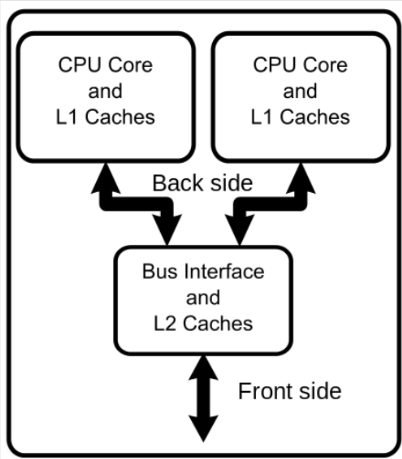
\includegraphics[width=0.8\textwidth]{fsbbsb}
    \centering
    \caption{Front side és back side buszok}
    \label{fig:fsbbsb}
\end{figure}

\subsection{FSB}
Az FSB két részre oszlik: északi és déli híd.
A north bridge gyorsabb, a memóriákkal és a grafikus interfésszel való kapcsolatot biztosítja (PCIe, AGP).
A south bridge (IO controller) a perifériákkal tartja a kapcsolatot (pl. PCI).
A vezérlők frekvenciája jelentősen kisebb a processzoránál, ezt a nagyobb sávszélességgel kompenzálja.

Később az északi hidat a processzorba integrálták.

\section{Fejlődés okai és irányai}
A buszrendszerek fejlődését a processzorok sebességének nagy léptékű fejlődése tette szükségessé.
Ezért a legfőbb cél az IO szűk keresztmetszet méréséklése.
Ennek érdekében bevezették a gyorsítótárakat és a blokkos adatátvitelt.

A processzorok fejlődésével nem tudtak lépést tartani a hagyományos párhuzamos buszok.
A probléma a perifériák csatlakoztatásánál is felmerült (pl. USB), sokszor az eszköz gyorsabb volt, mint amit a busz ki tudott szolgálni.

\section{IO eszközök és memória kapcsolata}
\begin{itemize}
    \item megosztott busz koncepció (pl. PCI)
    \item pont-pont kapcsolat, dedikált buszok (PCIe, HyperTransport, QPI)
\end{itemize}

\section{HyperTransport}
Az AMD fejlesztette ki ezt a buszrendszert 2001-ben.
Jellemzői:
\begin{itemize}
    \item kétirányú soros/párhuzamos kapcsolat
    \item alacsony késleltetés
    \item szélessávú kapcsolat
    \item rugalmas
    \item csomagokba ágyazza az adatokat
    \item 4, 8, 32 db soros vonalat tud kezelni
    \item általában CPU lapkára integrált, de nagy sávszélességű IO busznak is használják
    \item skálázható
    \item több csatorna alakítható ki
    \item erre csatlakozik az Ethernet, SATA, PCI, PCIe vezérlő is
    \item nem rendelkezik dedikált címtérrel, hanem a memóriában leképzett IO-val rendelkezik
\end{itemize}

Kétféle egységet tartalmaz:
\begin{itemize}
    \item tunnel
    \item cave - ez az utolsó egység, ez zárja le a HT láncot, amire a tunneleket fel lehet fűzni (max 4)
\end{itemize}

\section{QuickPath Interconnect}
Az Intel fejlesztése, feladata részben az FSB kiváltása volt.
2008-tól kezdték alkalmazni, először Xeon, később a Core i processzorokban is.
Lapkára integrált memóriavezérlővel és NUMA memóriahozzáféréssel rendelkezik.
Osztott memóriát használ, tehát a processzor 2 memóriavezérlővel rendelkezik és mindkettőhöz hozzá van csatlakoztatva 2-2 memória slot.
A processzor tehát nem mindegy, hogy melyik oldalról tölti be a memóriát.

A QPI is csomagkapcsolt rendszer, 5 rétegű architektúrát definiál (fizikai, kapcsolati, útválasztási, szállítási, protokoll).
2x20 vezetéket tartalmaz (adó és vevő).

Több processzoros rendszer esetén a QPI minden processzort minden processzorral összeköt.
